\documentclass[a4paper,10pt]{article}
\usepackage[utf8x]{inputenc}
\usepackage{graphics,graphicx}
\usepackage{longtable}
\usepackage{hyperref}
\usepackage{subcaption}
\renewcommand{\thefigure}{S\arabic{figure}}
\begin{document}

\section{Supplementary material}

Supplementary Figure S1: Example of a synthetic sample with high class imbalance. The three bars represent the different classes: loss, normal and gain. The y axis represents the number of probes in one class.
%\begin{figure*}[!h]
%\begin{center}
%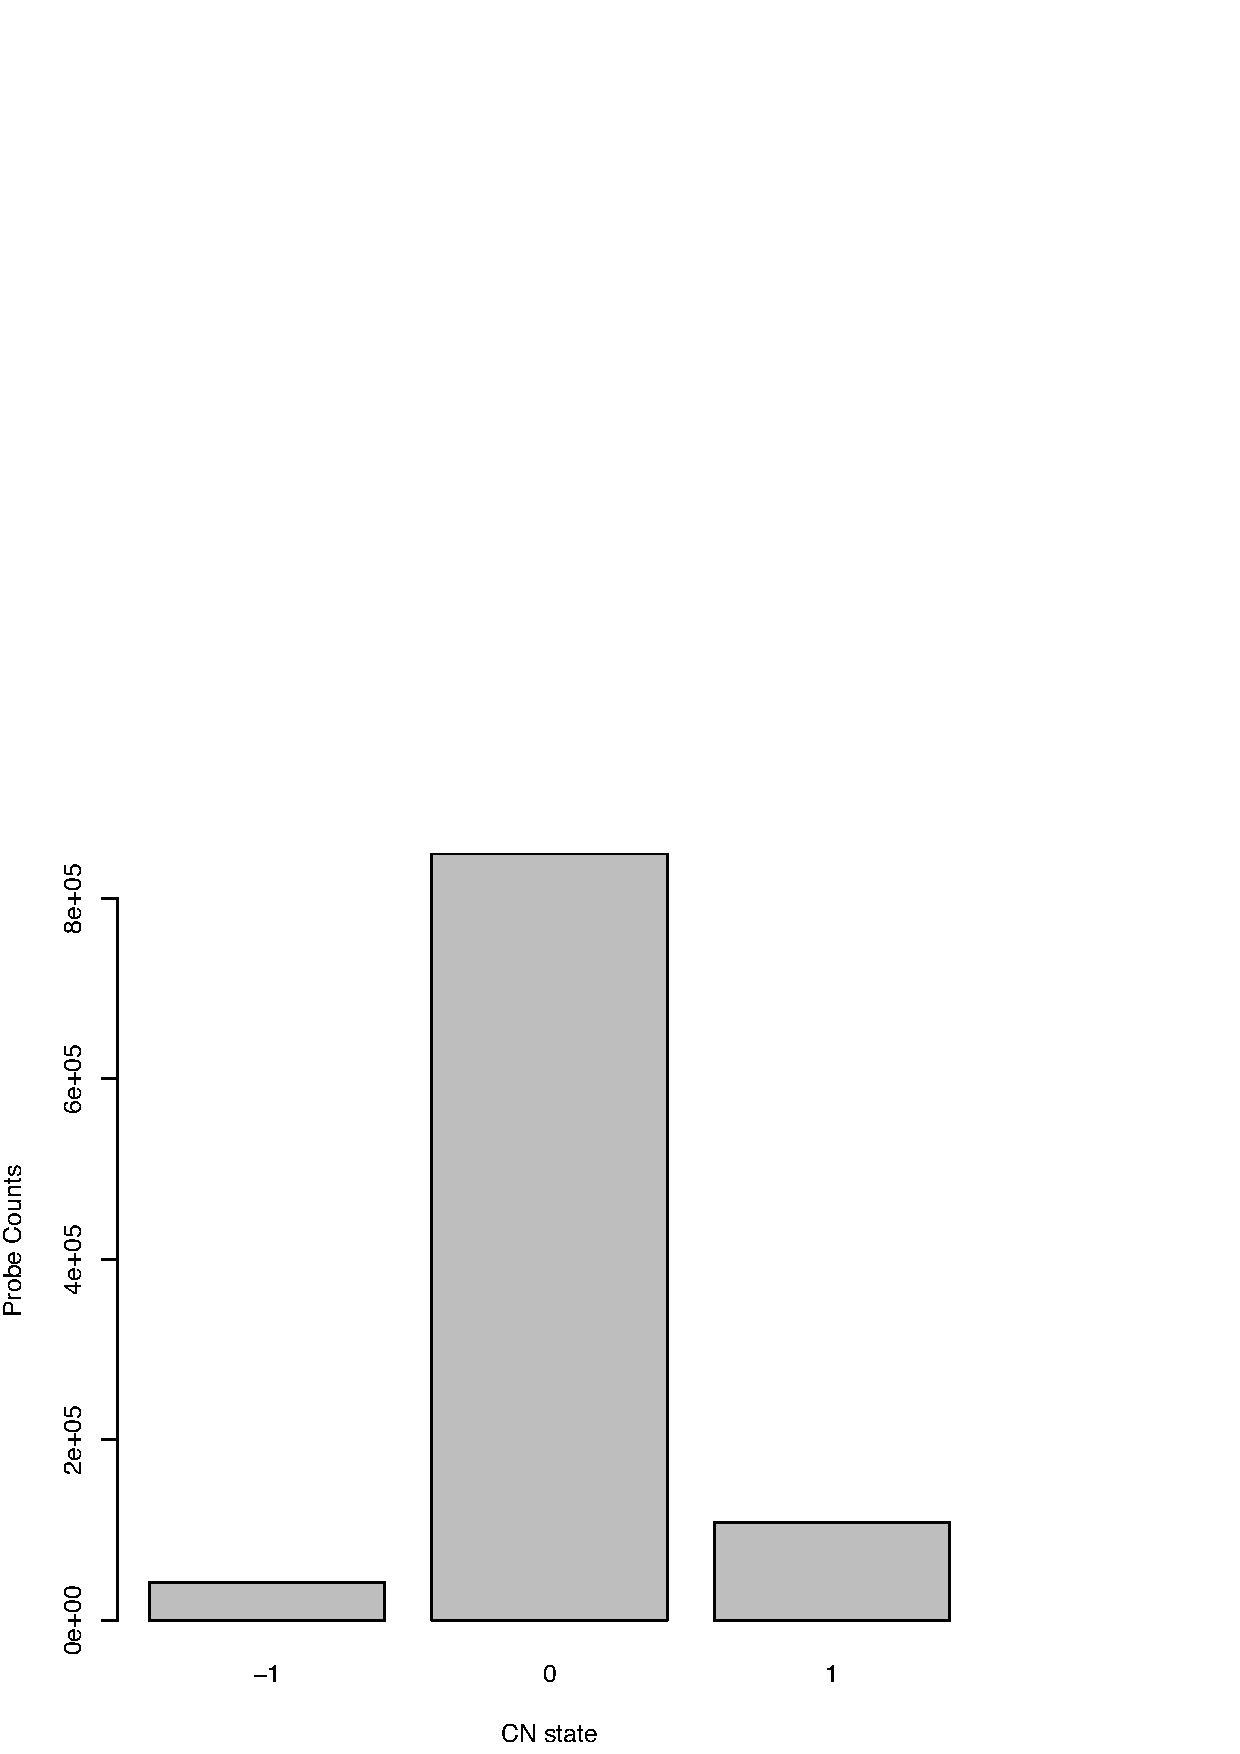
\includegraphics[width=\textwidth]{Figures/Supplementary_Figure_1.pdf}
%\end{center}
%\caption{Example of a synthetic sample with high class imbalance. The three bars represent the different classes: loss, normal and gain. The y axis represents the number of probes in one class.}
%\label{FigS1}	
%\end{figure*}


\noindent Supplementary Figure S2 shows the distribution of F-scores in synthetic samples with tumour purity 100\% for CGHcall and three adjusted versions of CGHcall. F-scores for different intervals used for normalization and postsegmentation normalization - CGHcall*. The y-axis represents the F-score. The three panels represent the three copy number states: loss, normal and gain.
%\begin{figure}[!t]
%\begin{center}
%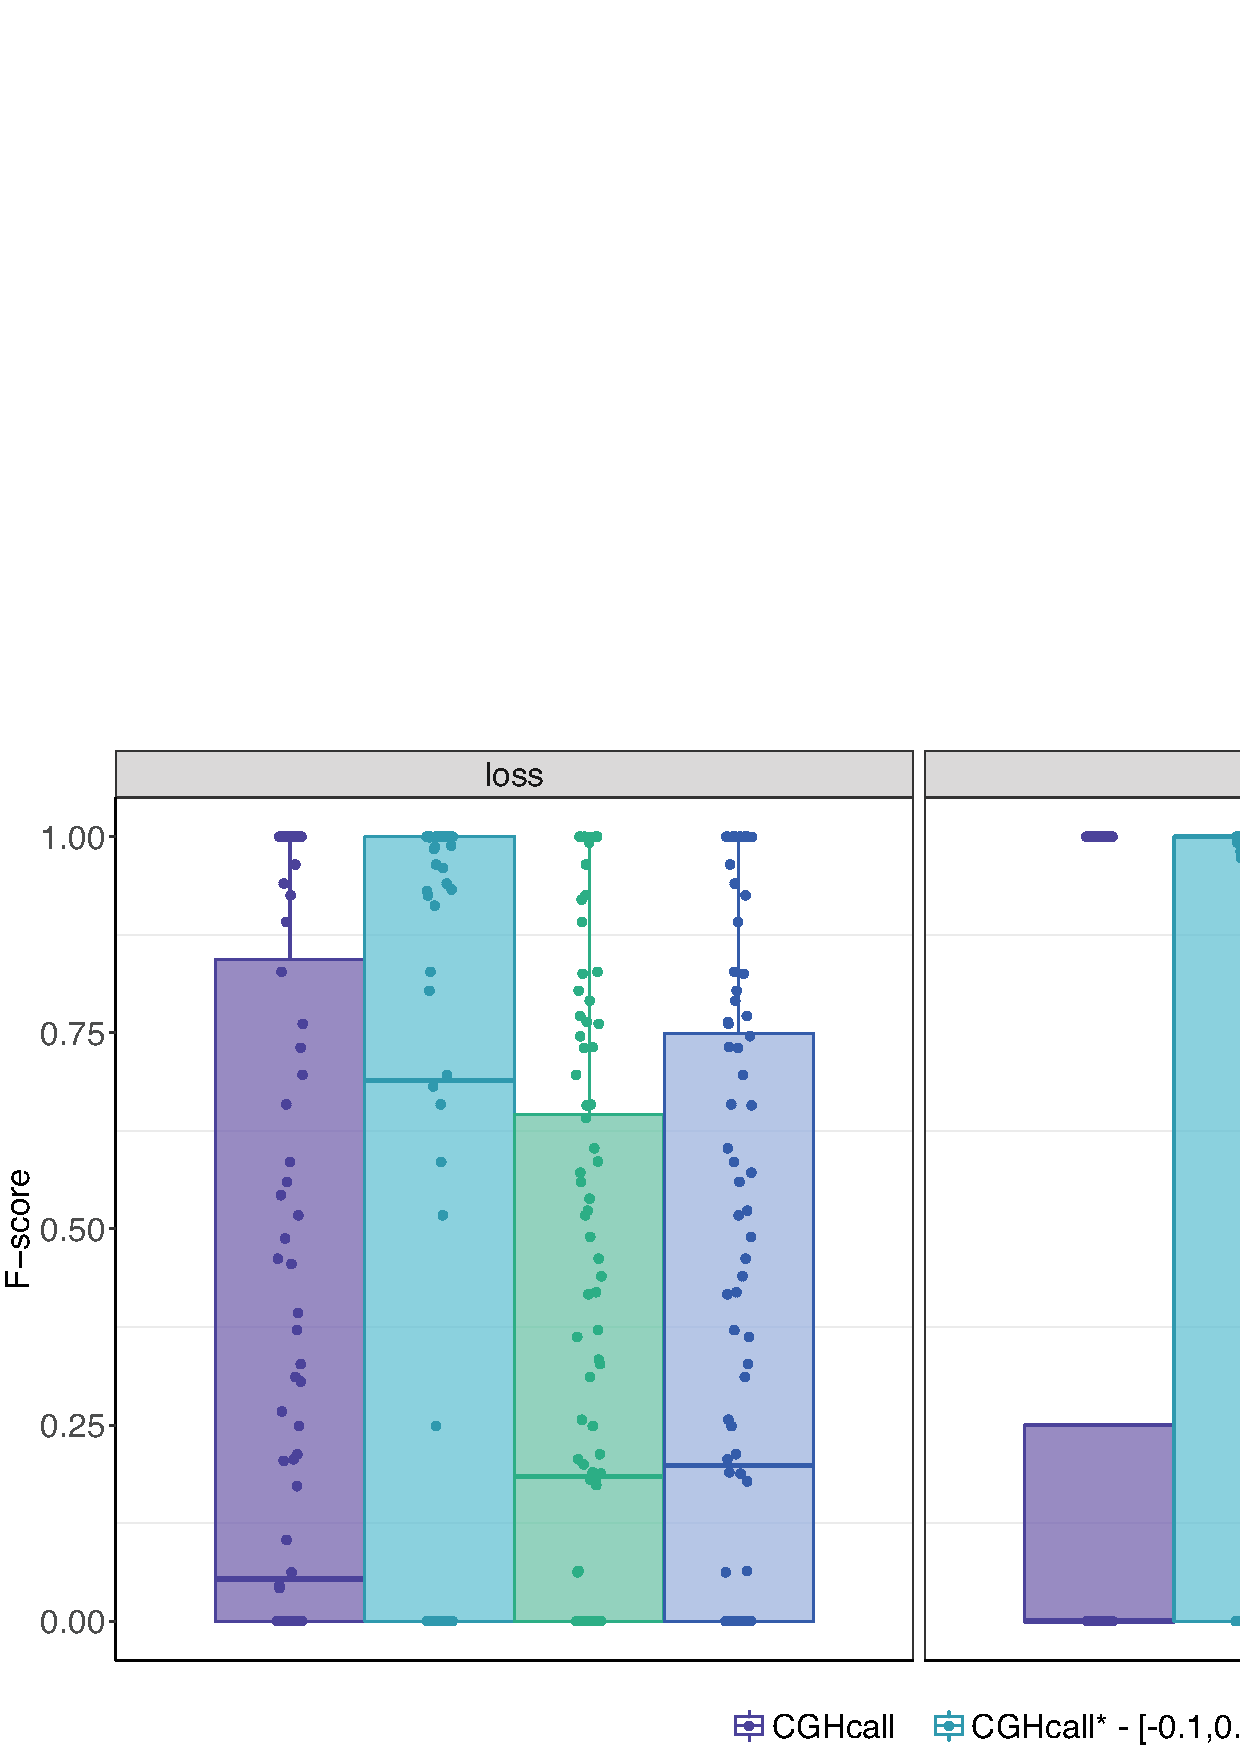
\includegraphics[width=\textwidth]{Figures/Supplementary_Figure_2.pdf}
%\end{center}
%\caption{F-scores for different intervals used for normalization and postsegmentation normalization - CGHcall*. The y-axis represents the F-score. The three panels represent the three copy number states: loss, normal and gain.}
%\label{FigS2}	
%\end{figure}


\end{document}

